\chapter{Instruction Selection \Author{D. Ebner \andAuthor A. Krall \andAuthor B. Scholz} \label{chapter:code_selection}}
\inputprogress
\graphicspath{{fig/}{code_selection/fig/}{part4/code_selection/fig/}}
% some frequently used macros
%%%%%%%%%%%%%%%%%%%%%%%%%%%%%%%%%%%%%%%%%%%%%%%%%%%%%%%%%%%%%%%%%%%%%
\newcommand{\cf}{c.f.\xspace}
\newcommand{\ea}{et~al.\xspace}

\newcommand{\preds}{\emph{preds}}
\newcommand{\succs}{\emph{succs}}
\newcommand{\costs}{\emph{costs}}
\newcommand{\tbd}[1]{\begin{itemize}\item#1\end{itemize}}
\newcommand\vardomain{\mathbb D}
\newcommand\matrixfont{\mathcal}
\newcommand\kw[1]{\textbf{#1}}

\newcommand\cfgnodes{\mathcal N}
\newcommand\cfgedges{\mathcal E}
\newcommand\cfgstart{\textbf{s}}
\newcommand\cfgend{\textbf{e}}
\newcommand\cfg{\textit{CFG}}
\newcommand\varset{\mathcal{V}}
\newcommand{\vdef}[1]{\cfgdef({#1})}
\newcommand{\defs}[1]{\mathcal{D}_{#1}}
\newcommand{\live}[1]{\mathcal{L}_{#1}}
\newcommand{\uses}[1]{\mathcal{U}_{#1}}
\newcommand{\pred}[2]{\cfgpred^{#1}_{#2}}
\newcommand\state{\textbf{state}}
\newcommand\bool{\mathbb B}
\newcommand\btrue{\textit{true}}
\newcommand\bfalse{\textit{false}}
\newcommand\transform{\mathbb T}
\newcommand\alive{\textbf{alive}}
\newcommand\Path{\textit{Path}}
\newcommand\Ops{\textit{Ops}}
\newcommand\bigo{\mathcal O}

\renewcommand{\vec}[1]{\overrightarrow{#1}}
\newcommand{\dotcup}{\ensuremath{\mathaccent\cdot\cup}}

% locally used colors (pantone)
%%%%%%%%%%%%%%%%%%%%%%%%%%%%%%%%%%%%%%%%%%%%%%%%%%%%%%%%%%%%%%%%%%%%%
\definecolor{LightBlue}{rgb}{ 0.67578125, 0.84375, 0.8984375 }
\definecolor{LightCoral}{rgb}{ 0.9375, 0.5, 0.5 }
\definecolor{LightCyan}{rgb}{ 0.875, 0.99609375, 0.99609375 }
\definecolor{LightGoldenRodYellow}{rgb}{ 0.9765625, 0.9765625, 0.8203125 }
\definecolor{LightGrey}{rgb}{ 0.82421875, 0.82421875, 0.82421875 }
\definecolor{LightGreen}{rgb}{ 0.5625, 0.9296875, 0.5625 }
\definecolor{LightPink}{rgb}{ 0.99609375, 0.7109375, 0.75390625 }
\definecolor{LightSalmon}{rgb}{ 0.99609375, 0.625, 0.4765625 }
\definecolor{LightSeaGreen}{rgb}{ 0.125, 0.6953125, 0.6640625 }
\definecolor{LightSkyBlue}{rgb}{ 0.52734375, 0.8046875, 0.9765625 }
\definecolor{LightSlateBlue}{rgb}{ 0.515625, 0.4375, 0.99609375 }
\definecolor{LightSlateGray}{rgb}{ 0.46484375, 0.53125, 0.59765625 }
\definecolor{LightSteelBlue}{rgb}{ 0.6875, 0.765625, 0.8671875 }
\definecolor{LightYellow}{rgb}{ 0.99609375, 0.99609375, 0.875 }
\definecolor{Orange}{rgb}{ 0.99609375, 0.64453125, 0.0 }
\definecolor{OrangeRed}{rgb}{ 0.99609375, 0.26953125, 0.0 }
\definecolor{Orchid}{rgb}{ 0.8515625, 0.4375, 0.8359375 }

% tikz styles
%%%%%%%%%%%%%%%%%%%%%%%%%%%%%%%%%%%%%%%%%%%%%%%%%%%%%%%%%%%%%%%%%%%%%
% \tikzstyle{arrow} = [draw,>=triangle 45]
% \tikzstyle{fnode} = [shape=ellipse, draw, minimum width=1.5cm,
%                      minimum height=0.8cm, node distance=1.5cm,
%                      text centered, fill=LightBlue]
\section{Introduction}

Instruction selection is a transformation step in a compiler that
translates a machine-independent intermediate code representation into
a low-level intermediate representation or to machine code for a
specific target architecture. Instead of hand-crafting an instruction
selector for each target architecture, generator tools have been
designed and implemented that generate the instruction selector based
on a specification of the target machine description of the
target. This approach is used in large compiler infrastructures such
as GCC or LLVM that target a range of architectures.  A possible
scenario of a code generator in a compiler is depicted in
Figure~\ref{fig:instruction-selection}. The Intermediate
Representation (IR) of an input program is passed on to an optional
lowering phase that breaks down instructions and performs other
machine dependent transformations. Thereafter, the instruction
selection performs the mapping to machine code or lowered IR based on
the machine description of the target architecture.


% \emph{3 pages}; introduction, related work
\begin{figure}[t]
  \begin{center}
%     \begin{tikzpicture}

%       \tikzstyle{fbox} = [rectangle, draw, sharp corners, text
%       width=2cm,minimum width=2.2cm, minimum height=1.3cm,text badly centered,
%       node distance=2.3cm, inner sep=2pt, fill=LightBlue]

%       \matrix [draw,column sep=0.6cm, inner sep=10pt,rounded corners] (matrix) {
%         \node [fbox] (lowering) {Lowering (optional)};
%         &
%         \node [fbox] (isel) {Instruction Selection};
%         \node [fbox, above of=isel, node distance=1.8cm] (mdesc) {Machine Description};
%         &
%         \node [fbox] (opts) {Machine-Dependent Backend}; \\
%       };

%       \path (matrix.north west) node [anchor=south west] {Code Generator};
%       \path [arrow,->] (lowering) -- node [above] {} (isel);
%       \path [arrow,->] (mdesc) -- (isel);
%       \path [arrow,->] (isel) -- node [above] {} (opts);
%       \path [arrow,<-] (lowering.west) -- +(-0.8cm,0cm) node [left] {IR};
%       \path [arrow,->] (opts.east) -- +(0.8cm,0cm) node [right, text width=1.5cm]
%       {Target Program};
%     \end{tikzpicture}
    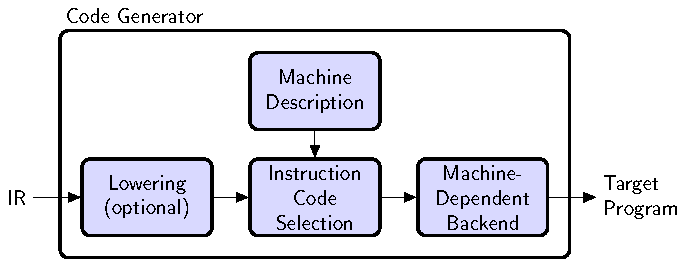
\includegraphics{pgf-fig001}
  \end{center}
  \caption{Scenario: An instruction selector translates a compiler's IR to a
    low-level machine-dependent representation.}
  \label{fig:instruction-selection}
\end{figure}

One of the widely used techniques in code generation is tree pattern
matching. Here, the unit of translation is a single statement
represented in the form of a data flow tree (DFT). The basic idea is
to describe the target instruction set using an \emph{ambiguous}
cost-annotated graph grammar. The instruction selector seeks for a
cost-minimal \emph{cover} of the DFT. Each of the selected rules have
an associated semantic action that is used to emit the corresponding
machine instructions, either by constructing a new intermediate
representation or by rewriting the DFT bottom-up.
\begin{figure}[ht]
  \begin{center}
%     \begin{tikzpicture}
%       \node at (0,0) [fnode] (rega) {\texttt{VAR:a} };
%       \node at (2,0) [fnode] (regi) {\texttt{VAR:i} };
%       \node at (4,0) [fnode] (cst2) {\texttt{CST:2} };

%       \path (cst2) ++(240:2cm) node[fnode] (shl) {\texttt{SHL} } ;
%       \path (shl) ++(240:1.5cm) node[fnode] (add) {\texttt{ADD} } ;
%       \path (add) ++(270:1.5cm) node[fnode] (ldw) {\texttt{LD} } ;

%       \path[arrow,->] (regi) edge (shl);
%       \path[arrow,->] (cst2) edge (shl);
%       \path[arrow,->,bend left=15] (shl) edge (add);
%       \path[arrow,->,bend right=15] (rega) edge (add);
%       \path[arrow,->] (add) edge (ldw);

%       \node at (-2.8,-2.8) (rega) {
%         \begin{minipage}[]{7cm}
% \begin{verbatim}
% s   <- reg                : 0
% reg <- imm                : 1
% imm <- IMM                : 0
% reg <- VAR                : 0
% reg <- SHL(reg, reg)      : 1
% reg <- SHL(reg, imm)      : 1
% reg <- ADD(reg, reg)      : 1
% reg <- LD(reg)            : 1
% reg <- LD(ADD(reg, reg))  : 1
% reg <- LD(ADD(reg, SHL(reg, imm))) : 1
% \end{verbatim}
%         \end{minipage}
%       };
%     \end{tikzpicture}
    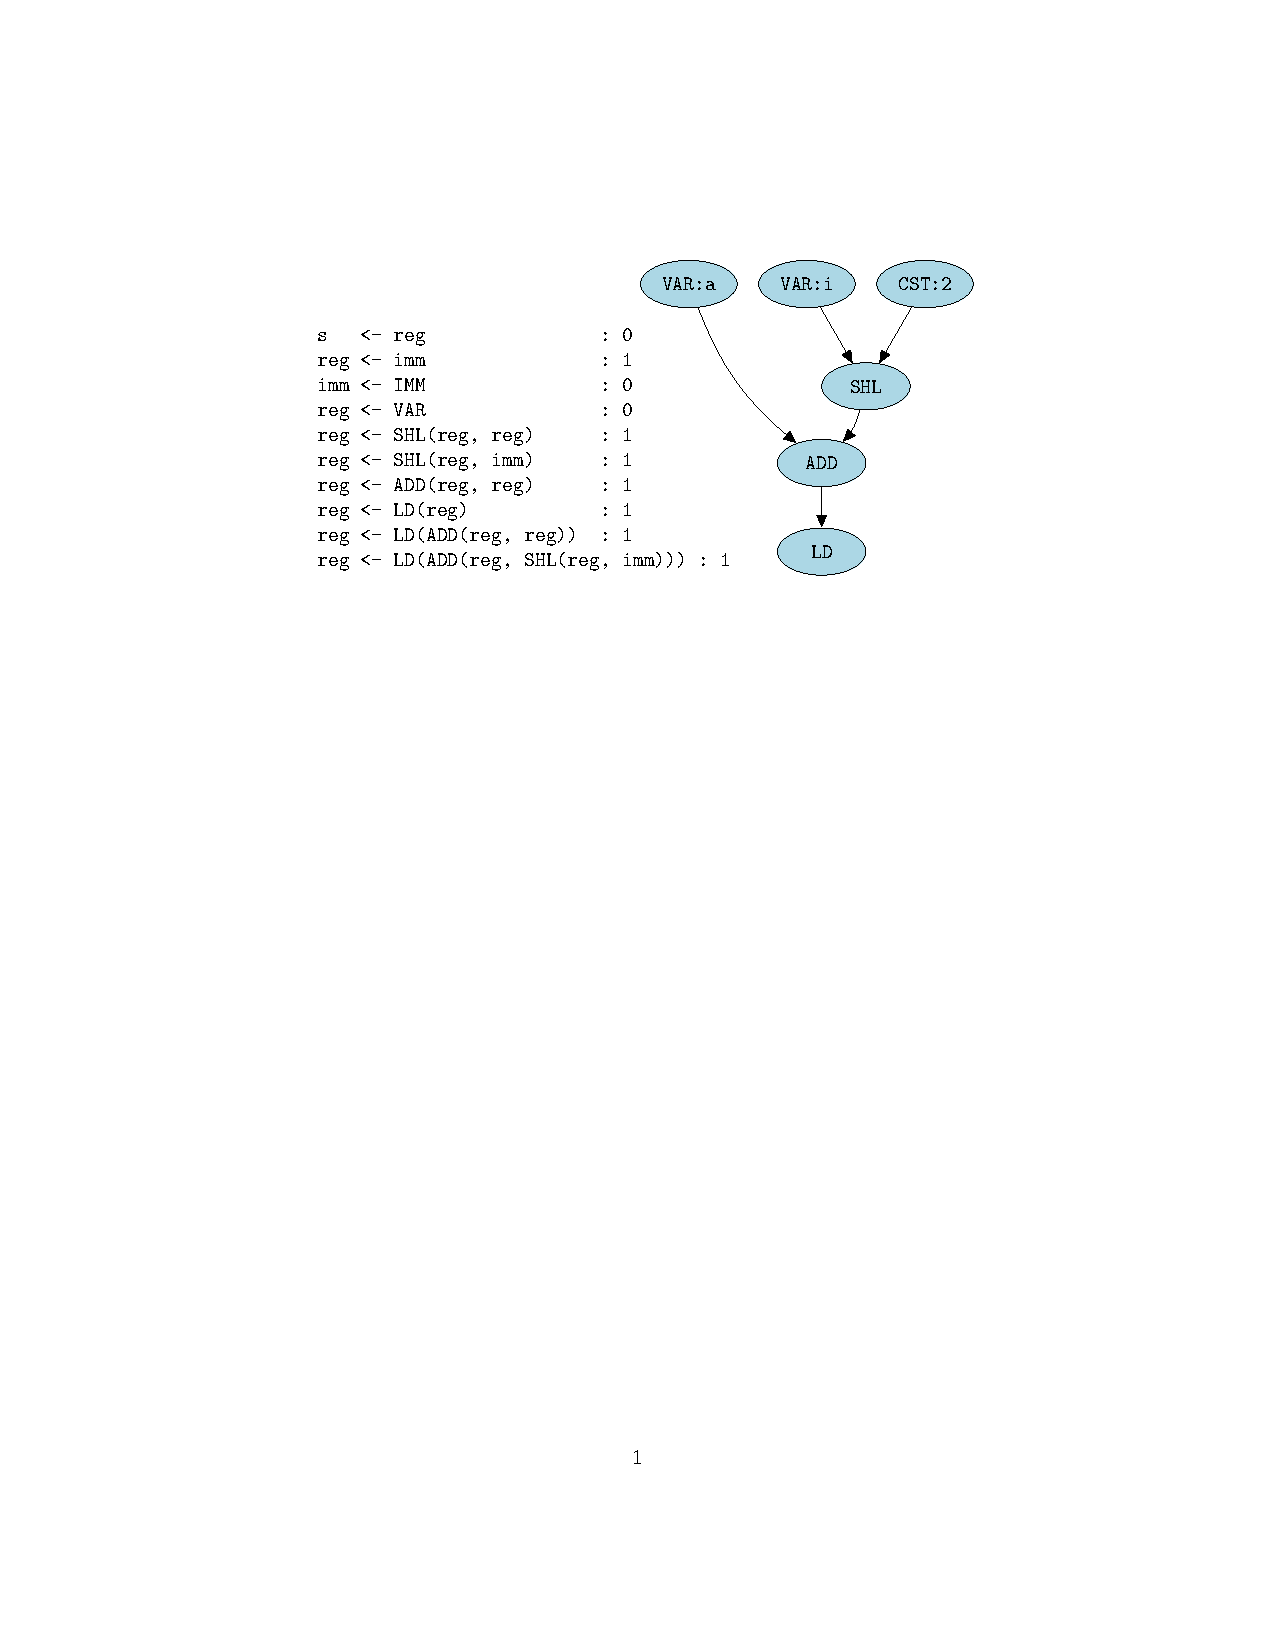
\includegraphics{pgf-fig002}
  \end{center}
  \caption{Example of a data flow tree and a rule fragment with
    associated costs.}\label{fig:tpm}
\end{figure}

An example of a DFT along with a set of rules representing valid ARM
instructions is shown in Figure~\ref{fig:tpm}. Each rule consists of
nonterminals (shown in lower-case), and terminal symbols (shown in
upper-case). Nonterminals are used to chain individual rules together.
Nonterminal \texttt{s} denotes a distinguished start symbol for the
root node of the DFT. Terminal symbols match the corresponding labels
of nodes in the dataflow trees. The terminals of the grammar are
\texttt{VAR}, \texttt{CST}, \texttt{SHL}, \texttt{ADD}, and
\texttt{LD}.  Rules that translate from one nonterminal to another are
called \emph{chain rules}, e.g., \texttt{reg <- imm} that translates
an immediate value to a register. Note that there are multiple
possibilities to obtain a cover of the data-flow tree for the example
shown in Figure~\ref{fig:tpm}.  Each rule has associated costs. The
cost of a tree cover is the sum of the costs of the selected
rules. For example, the DFT could be covered by rules (3), (4), and
(11) which would give a total cost for the cover of one cost
unit. Alternatively, the DFT could be covered by rule (2), (6), (8),
and (9) which yields 4 cost units for the cover for issuing 4 assembly
instructions. A dynamic programming algorithm selects a cost optimal
cover for the DFT.

\begin{figure}[ht]
  \begin{center}
%     \begin{tikzpicture}
%       \node [anchor=south west] at (-4cm, 0cm) (listing) {
%         \lstset {
%           language=C,
%           basicstyle=\footnotesize,
%           morekeywords={fract_t, _Fract},
%         }
%         \begin{lstlisting}
% typedef unsigned _Fract short fract_t;
% fract_t dot_product(fract_t *p, fract_t *q) {
%   fract_t s = 0, *e = p + N;
%   while(p < e) s += *p++ * *q++;
%   return s;
% }
%        \end{lstlisting}
%       };

%       \node [fnode, fill=LightGreen] (ret) {\texttt{ret}};
%       \node [fnode, fill=LightGreen, below of=ret] (phi1) {$\phi$};
%       \node [fnode, below of=phi1] (add1) {\texttt{ADD}};
%       \node [fnode, below of=add1] (mul) {\texttt{MUL}};
%       \node [fnode, right of=mul, node distance=2cm] (phi3) {$\phi$};
%       \node [fnode, fill=LightYellow, below right of=phi3, node distance=2cm]
%             (cst0) {\texttt{CST:0}};
%       \path[arrow,->] (mul) edge (add1);
%       \path[arrow,->] (add1) edge (phi1);
%       \path[arrow,->] (phi1) edge (ret);

%       \node [fnode] at ($(mul)+(-1.7cm,-1.5cm)$) (ldp) {\texttt{LD}};
%       \node [fnode, below left of=ldp, node distance=2cm] (phip) {$\phi$};
%       \node [fnode, fill=LightYellow] at ($(phip)+(-1.5cm,-1.5cm)$) (varp) {\texttt{VAR:p}};
%       \node [fnode] at ($(phip)+(+1.5cm,-1.5cm)$) (inc) {\texttt{INC}};
%       \path[arrow,->] (varp) -- (phip);
%       \path[arrow,->] (inc) -- (phip);
%       \path[arrow,->] (phip) -- (ldp);
%       \path[arrow,->, bend left=5] (ldp) edge (mul);
%       \path [arrow,->] (phip) .. controls ($(phip.east)+(2cm,0cm)$)
%             and ($(inc.east)+(1cm,-1.5cm)$) .. (inc);

%       \node [fnode] at ($(mul)+(1.7cm,-1.5cm)$) (ldq) {\texttt{LD}};
%       \node [fnode, below right of=ldq, node distance=2cm] (phiq) {$\phi$};
%       \node [fnode] at ($(phiq)+(-1.5cm,-1.5cm)$) (varq) {\texttt{VAR:q}};
%       \node [fnode] at ($(phiq)+(+1.5cm,-1.5cm)$) (inc) {\texttt{INC}};
%       \path[arrow,->] (varq) -- (phiq);
%       \path[arrow,->] (inc) -- (phiq);
%       \path[arrow,->] (phiq) -- (ldq);
%       \path[arrow,->, bend right=5] (ldq) edge (mul);
%       \path [arrow,->] (phiq) .. controls ($(phiq.east)+(2cm,0cm)$)
%             and ($(inc.east)+(1cm,-1.5cm)$) .. (inc);

%       \node [fnode] at ($(phip)+(0.5cm,4.5cm)$) (lt) {\texttt{<}};
%       \node [fnode, fill=LightYellow, below left of=lt,
%              node distance=2cm] (add) {\texttt{ADD}};
%       \node [fnode, fill=LightYellow, below of=add] (cstn) {\texttt{CST:2N}};
%       \path[arrow,->, bend left=5] (add) edge (lt);
%       \path[arrow,->] (varp) ..controls ($(cstn)+(-1.5cm,0)$) .. (add);
%       \path[arrow,->] (cstn) -- (add);
%       \path[arrow,->, bend left=5] (phip) edge (lt);
%       \path[arrow,->, bend right=5] (phi3) edge (add1);
%       \path[arrow,->] (add1) .. controls ($(add1.east)+(2cm,0cm)$)
%             and ($(phi3.east)+(2cm,-1cm)$) .. (phi3);
%       \path[arrow,->] (cst0) .. controls ($(phi3.east)+(1.5cm,0cm)$) ..  (phi1);
%       \path[arrow,->,bend right=5] (cst0) edge (phi3);

%     \end{tikzpicture}

    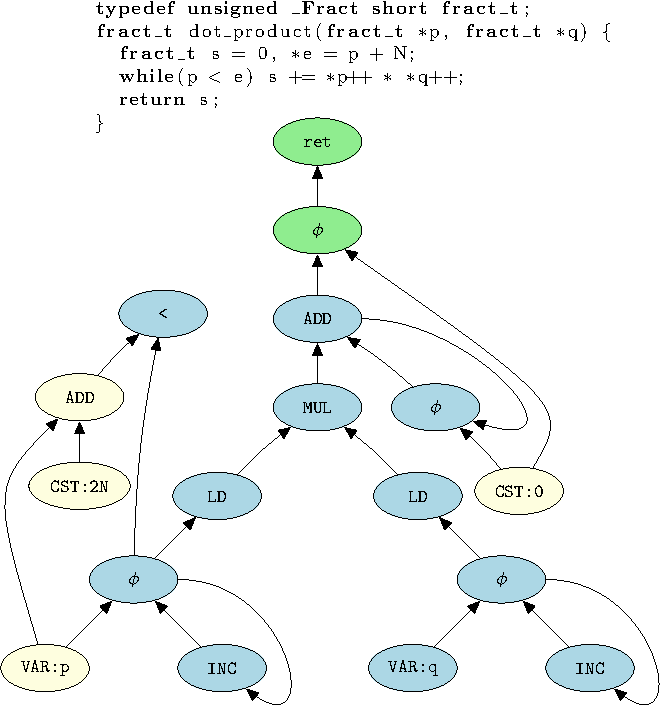
\includegraphics{pgf-fig003}
  \end{center}
  \caption{Instruction selection DAG for a vector dot-product in
    fixed-point artithmetic.}\label{fig:ssa_graph}
\end{figure}

Tree pattern matching on a DFT is limited to the scope of a single
statement.  To overcome this limitation, we can extend the scope of
the matching algorithm to the computational flow of a whole procedure.
The use of the Static Single Assignment (SSA) form as an intermediate
representation improves the code generation by making def-use
relationships explicit. Hence, SSA exposes the data flow of a
translation unit and utilizes the code generation process.  Instead of
using a textual SSA representations, we employ a graph representation
of SSA called the \emph{SSA graph} that is an extension of DFTs and
represents the data-flow of a procedure in SSA form.  SSA graphs are a
suitable representation for code generation: First, SSA graphs capture
acyclic and cyclic information flow beyond basic block
boundaries. Second, SSA graphs often arise naturally in modern
compilers as the intermediate code representation usually already is
in SSA form. Third, output or anti-dependencies in SSA graph do not
exist.

As SSA graphs are potentially cyclic, no dynamic programming approach
can be employed for instruction selection.  To get a handle on code
selection for SSA graphs, we will discuss in the following an approach
based on a reduction to a quadratic mathematical programming problem
(PBQP) that has been adopted by at least two major embedded system
compiler vendors.  Consider the code fragment of a dot-product routine
and the corresponding SSA graph shown in Figure~\ref{fig:ssa_graph}.
The code implements a simple vector dot-product using fixed-point
arithmetic in Embedded~C.  Nodes in the SSA graph represent a single
operation while edges describe the flow of data that is produced at the
source node and consumed at the target node. Incoming edges
have an order which reflects the argument order of the operation. In
the figure the color of the nodes indicates to which basic block the
operations belong to.

The example in Figure~\ref{fig:ssa_graph} has fixed-point computations
that need to be modelled in the grammar. For fixed-point values most
arithmetic and bitwise operations are identical to their integer
equivalents. However, some operations have different semantics, \eg
multiplying two fixed-point values in format $m.i$ results in a value
with $2*i$ fractional digits. The result of the multiplication has to
be adjusted by a shift operation to the right. To accommodate for
fixed-point values, we add the following rules to the grammar
introduced in Figure~\ref{fig:tpm}:
\begin{alltt}
   reg <- VAR : is\_fixed_point() ? \(\infty\) : 0
   fp  <- VAR : is\_fixed_point() ? 0 : \(\infty\)
   fp2 <- MUL(fp, fp)   : 1   \{ MUL Rd, Rm, Rs \}
   fp  <- fp2           : 1   \{ LSR Rd, Rm, i  \}
   fp  <- ADD(fp, fp)   : 1   \{ ADD Rd, Rm, Rs \}
   fp2 <- ADD(fp2, fp2) : 1   \{ ADD Rd, Rm, Rs \}
   fp  <- PHI(fp, ...) : 0 
   fp2 <- PHI(fp2, ...) : 0 
\end{alltt}

In the example the accumulation for double-precision fixed
point values can be performed at the same cost as for \texttt{fp}. Thus, it would be
beneficial to move the necessary shift from the inner loop to the
return block, performing the intermediate calculations in the extended
format. However, as a tree-pattern matcher generates code at 
statement-level, the information of having values as double-precision
cannot be hoisted across basic block boundaries.
An instruction selector that is operating on the SSA graph, is able to propagate 
nonterminal \texttt{fp2} across the $\phi$ node prior to the return 
and emits the code for the shift to the right in the return block.

In the following, we will explain how to perform instruction selection
on SSA graphs with the means of a specialized quadratic assignment
problem (PBQP). First, we discuss the instruction selection problem by
employing a discrete optimisation problem called partitioned boolean
quadratic problem.  An extension of \emph{patterns} to arbitrary
acyclic graph structures, which we refer to as DAG grammars, is
discussed in Sub-Section~\ref{sec:dag_patterns}. As we move from
acyclic linear code regions to whole-functions, it becomes less
clear in which basic block, the selected machine instructions should
be emitted. For chain rules, the obvious choices are often
sub-optimal. We will discuss in Section~\ref{sec:chain_rule_placement}
a polynomial-time algorithm based on generic network flows that can be
applied to generate more efficient code based on a flexible cost
model.

\section{Code Selection for Tree Patterns on SSA-Graphs}
% \emph{5 pages}; modeling, continued example
The matching problem for SSA graphs reduces to a discrete optimization
problem called Partitioned Boolean Quadratic Problem (PBQP).  First,
we will introduce the PBQP problem and then we will describe the
mapping of the instruction selection problem to PBQP.

\subsection{Partitioned Boolean Quadratic Problem}
\label{sec:pbqp}
% \emph{2 pages}; introduction into PBQP, algorithms, and applications
Partitioned Boolean Quadratic Programming (PBQP) is a generalized
quadratic assignment problem that has proven to be effective for a
wide range of applications in embedded code generation, \eg
instruction selection, register assignment, address mode selection, or
bank selection for architectures with partitioned memory. Instead of
problem-specific algorithms, these problems can be modeled in terms of
generic {PBQP}s that are solved using a common solver library. PBQP is
flexible enough to model irregularities of embedded architectures that
are hard to cope with using traditional heuristic approaches.

Consider a set of discrete variables $X=\{x_1,\ldots,x_n\}$ and their
finite domains $\{\vardomain_1,\ldots,\vardomain_n\}$. A solution of
PBQP is a mapping $h$ of each variable to an element in its domain,
i.e., an element of $\vardomain_i$ needs to be chosen for variable
$x_i$. The chosen element imposes local costs and costs between a
neighbour variable which we refer to as related costs.  Hence, the
quality of a solution is based on the contribution of two sets of
terms.
\begin{enumerate}
\item For assigning variable $x_i$ to the element $d_i$ in
  $\vardomain_i$. The quality of the assignment is measured by a
  \emph{local cost function} $c(x_i, d_i)$.
\item For assigning two related variables $x_i$ and $x_j$ to the
  elements $d_i \in \vardomain_i$ and $d_j \in \vardomain_j$.  We
  measure the quality of the assignment with a \emph{related cost
    function\/} $C(x_i,x_j, d_i,d_j)$.
\end{enumerate}
The total cost of a solution $h$ is given as,
\begin{equation}
  f\! =\! \sum_{1 \leq i \leq n} \hspace{-1mm} c(x_i,h(x_i)) + \hspace{-3mm} \sum_{1 \leq i < j  \leq n} \hspace{-3.5mm}
  C\left (x_i,x_j, h(x_i), h(x_j) \right). \label{eqn-pbqp}
\end{equation}
The PBQP problem seeks for an assignment of variables $x_i$ with
minimum total costs.

In the following we represent both the local cost function and the
related cost function in matrix form, i.e., the related cost function
$C(x_i,x_j,d_i,d_j)$ is decomposed for each pair $(x_i,x_j)$. The
costs for the pair are represented as matrix/table ${\matrixfont
  C}_{ij}$. A matrix element corresponds to an assignment $(d_i,
d_j)$. Similarly, the local cost function $c(x_i,d_i)$ is represented
by a cost vector $\vec{c_i}$ enumerating the costs of the elements.  A
PBQP problem has an underlying graph structure graph $G=(V,E,C,c)$,
which we refer to as a PBQP graph. For each decision variable $x_i$ we
have a corresponding node $v_i \in V$ in the graph, and for each cost
matrix ${\matrixfont C}_{i,j}$ that is not the zero matrix, we
introduce an edge $e=(v_i,v_j)$. The cost functions $c$ and $C$ map
nodes and edges to the original cost vectors and matrices
respectively.  We will present an example later in this chapter in the
context of instruction selection.

In general, finding a solution to this minimization problem is NP
hard.  However, for many practical cases, the PBQP instances are
sparse, \ie many of the cost matrices ${\matrixfont C}_{i,j}$ are zero
matrices and do not contribute to the overall solution. Thus, optimal
or near-optimal solutions can often be found within reasonable time
limits.  Currently, there are two algorithmic approaches for PBQP that
have been proven to be efficient in practice for instruction selection
problems, \ie a polynomial-time heuristic algorithm and a
branch-\&-bound based algorithm with exponential worst case
complexity.  For a certain subclass of PBQP, the algorithm produces
provably optimal solutions in time ${\cal O}(n m^3)$, where $n$ is the
number of discrete variables and $m$ is the maximal number of elements
in their domains, \ie $m=\max
\left(|\vardomain_1|,\ldots,|\vardomain_n\right|)$. For general
{PBQP}s, however, the solution may be sub-optimal. To obtain still an
optimal solution outside the sub-class, branch-\&-bound techniques can
be applied.

\subsection{Code Selection with PBQP}
In the following, we describe the modelling of code selection for SSA
graphs as a PBQP problem.  In the basic modeling, SSA and PBQP graphs
coincide.  The variables $x_i$ of the PBQP are decision variables
reflecting the choices of applicable rules (represented by
$\vardomain_i$) for the corresponding node of $x_i$. The local costs
reflect the costs of the rules and the related costs reflect the costs
of chain rules making rules compatible with each other.  This means
that the number of decision vectors and the number of cost matrices in
the PBQP are determined by the number of nodes and edges in the SSA
graph respectively.  The sizes of $\vardomain_i$ depend on the number
of rules in the grammar. A solution for the PBQP instance induces a
complete cost minimal cover of the SSA graph.

As in traditional tree pattern matching, an ambiguous graph grammar
consisting of tree patterns with associated costs and semantic actions
is used. Input grammars have to be \emph{normalized}. This means that
each rule is either a so-called \emph{base rule} or a \emph{chain
  rule}. A base rule is a production of the form $\texttt{nt}_0
\leftarrow \textit{op} ( \texttt{nt}_1, \dots, \texttt{nt}_{k_p} )$
where $\texttt{nt}_i$ are non-terminals and $\textit{op}$ is a
terminal symbol, \ie an operation represented by a node in the SSA
graph. A chain-rule is a production of the form $\texttt{nt}_0
\leftarrow \texttt{nt}_1$, where $\texttt{nt}_0$ and $\texttt{nt}_1$
are non-terminals.  A production rule $\texttt{nt} \leftarrow
\textit{op}_1 ( \alpha, \textit{op}_2 (\beta), \gamma))$ can be
normalized by rewriting the rule into two production rules
$\texttt{nt} \leftarrow \textit{op}_1 ( \alpha, \texttt{nt}' ,
\gamma)$ and $\texttt{nt}' \leftarrow \textit{op}_2 ( \beta)$ where
$\texttt{nt}'$ is a new non-terminal symbol and $\alpha,\beta$ and
$\gamma$ denote arbitrary pattern fragments.  This transformation can
be iteratively applied until all production rules are either chain
rules or base rules.  To illustrate this transformation, consider the
grammar in Figure~\ref{fig:pbpq-example}, which is a normalized
version of the tree grammar introduced in
Figure~\ref{fig:tpm}. Temporary nonterminal symbols $\texttt{t1}$,
$\texttt{t2}$, and $\texttt{t3}$ are used to decompose larger tree
patterns into simple base rules. Each base rule spans across a single
node in the SSA graph.


\begin{figure}
  \begin{center}
%     \begin{tikzpicture}
%       \tikzstyle{arrow} = [draw,>=triangle 45]
%       \tikzstyle{tarrow} = [arrow,thick]

%       \path (275:11cm) node[draw,shape=rectangle,fill=LightBlue]
%       {
%         \begin{minipage}{5.2cm}
%           \small
%           \begin{tabular}{l|l}
%             $R_1$ & \texttt{{imm} <- IMM}\\
%             $R_2$ & \texttt{reg <- VAR}\\
%             $R_3$ & \texttt{reg <- imm}\\
%             $R_4$ & \texttt{reg <- SHL(reg, {reg})}\\
%             $R_5$ & \texttt{reg <- SHL(reg, imm)}\\
%             $R_6$ & \texttt{t1 \ <- SHL(reg, imm)}\\
%             $R_7$ & \texttt{reg <- ADD(reg, reg)}\\
%             $R_8$ & \texttt{t2 \ <- ADD(reg, t1)}\\
%             $R_9$ & \texttt{t3 \ <- ADD(reg, reg)}\\
%             $R_{10}$ & \texttt{reg <- LDW(reg)}\\
%             $R_{11}$ & \texttt{reg <- LDW(t2)}\\
%             $R_{12}$ & \texttt{reg <- LDW(t3)}
%           \end{tabular}
%         \end{minipage}
%       }
%       ;

%       \tikzstyle{every node}=[minimum size=1.3cm];

%       \path (0:0) node[draw,shape=circle,fill=LightBlue]
%       (rega) {\small\texttt{VAR:a} }
%       node[right=14pt] {
%         \small
%         $\begin{array}{ccc}
%           & \color{OrangeRed}R_2 &  \\ \cline{2-2}
%           ( & \color{OrangeRed}0 & )
%         \end{array}$
%       }
%       node[right=3cm,draw,shape=circle,fill=LightBlue] (regi) {\small\texttt{VAR:i}}
%       node[right=4.3cm] {
%         \small
%         $\begin{array}{ccc}
%           & \color{OrangeRed}R_2 &  \\ \cline{2-2}
%           ( & \color{OrangeRed}0 & )
%         \end{array}$
%       }
%       node[right=8cm,draw,shape=circle,fill=LightBlue] (cst2) {\small\texttt{CST:2}}
%       node[right=9.3cm] {
%         \small
%         $\begin{array}{ccc}
%           & \color{OrangeRed}R_1 &  \\ \cline{2-2}
%           ( & \color{OrangeRed}0 & )
%         \end{array}$
%       };

%       \path (cst2) ++(250:4cm) node[draw,shape=circle,fill=LightBlue]
%       (shl) {\small\texttt{SHL} }
%       node[right=14pt] {
%         \small
%         $\begin{array}{ccccc}
%           & R_4 & R_5 & \color{OrangeRed}R_6 & \\ \cline{2-4}
%           ( & 1 & 1 & \color{OrangeRed}0 & )
%         \end{array}$
%       };

%       \path (shl) ++(250:5cm) node[draw,shape=circle,fill=LightBlue]
%       (add) {\small\texttt{ADD} }
%       node[right=14pt] {
%         \small
%         $\begin{array}{ccccc}
%           & R_7 & \color{OrangeRed}R_8 &  R_9 & \\ \cline{2-4}
%           ( & 1 & \color{OrangeRed}0 & 0 & )
%         \end{array}$
%       };

%       \path (add) ++(270:4cm) node[draw,shape=circle,fill=LightBlue]
%       (ldw) {\small\texttt{LDW} }
%       node[right=14pt] {
%         \small
%         $\begin{array}{ccccc}
%           & R_{10} & \color{OrangeRed}R_{11} & R_{12} &  \\ \cline{2-4}
%           ( & 1 & \color{OrangeRed}1 & 1 & )
%         \end{array}$
%       };

%       \path[tarrow,->, bend right=15] (regi) edge
%       node[left=-30pt,fill=white] {
%         \small
%         $\begin{array}{l|ccc}
%           & \texttt{reg} & \texttt{reg} & \color{OrangeRed}\texttt{reg}\\ \hline
%           \color{OrangeRed}\texttt{reg} & 0 & 0 & \color{OrangeRed}0\\
%         \end{array}$}
%       (shl);

%       \path[tarrow,->, bend left=15] (cst2) edge
%       node[right=-35pt,fill=white] {
%         \small
%         $\begin{array}{l|ccc}
%           & \texttt{reg} & \texttt{imm} & \color{OrangeRed}\texttt{imm}\\ \hline
%             \color{OrangeRed}\texttt{imm} & 1 & 0 & \color{OrangeRed}0\\
%         \end{array}$}
%       (shl);

%       \path[tarrow,->,bend left=15] (shl) edge
%       node[right=-30pt,fill=white] {
%         \small
%         $\begin{array}{l|ccc}
%           & \texttt{reg} & \color{OrangeRed}\texttt{t1} & \texttt{reg}\\ \hline
%           \texttt{reg} & 0 & \infty & 0\\
%           \texttt{reg} & 0 & \infty & 0\\
%           \color{OrangeRed}\texttt{t1} & \infty & \color{OrangeRed}0 & \infty\\
%         \end{array}$}
%       (add);

%       \path[tarrow,->,bend right=15] (rega) edge
%       node[fill=white] {
%         \small
%         $\begin{array}{l|ccc}
%           & \texttt{reg} & \color{OrangeRed}\texttt{reg} & \texttt{reg}\\ \hline
%           \color{OrangeRed}\texttt{reg} & 0 & \color{OrangeRed}0 & 0\\
%         \end{array}$}
%       (add);

%       \path[tarrow,->] (add) edge
%       node[right=2pt,fill=white] {
%         \small
%         $\begin{array}{l|ccc}
%           & \texttt{reg} & \color{OrangeRed}\texttt{t2} & \texttt{t3}\\ \hline
%           \texttt{reg} &0 & \infty & \infty \\
%           \color{OrangeRed}\texttt{t2} &\infty & \color{OrangeRed}0 & \infty \\
%           \texttt{t3} &\infty & \infty & 0\\
%         \end{array}$}
%       (ldw);

%     \end{tikzpicture}
    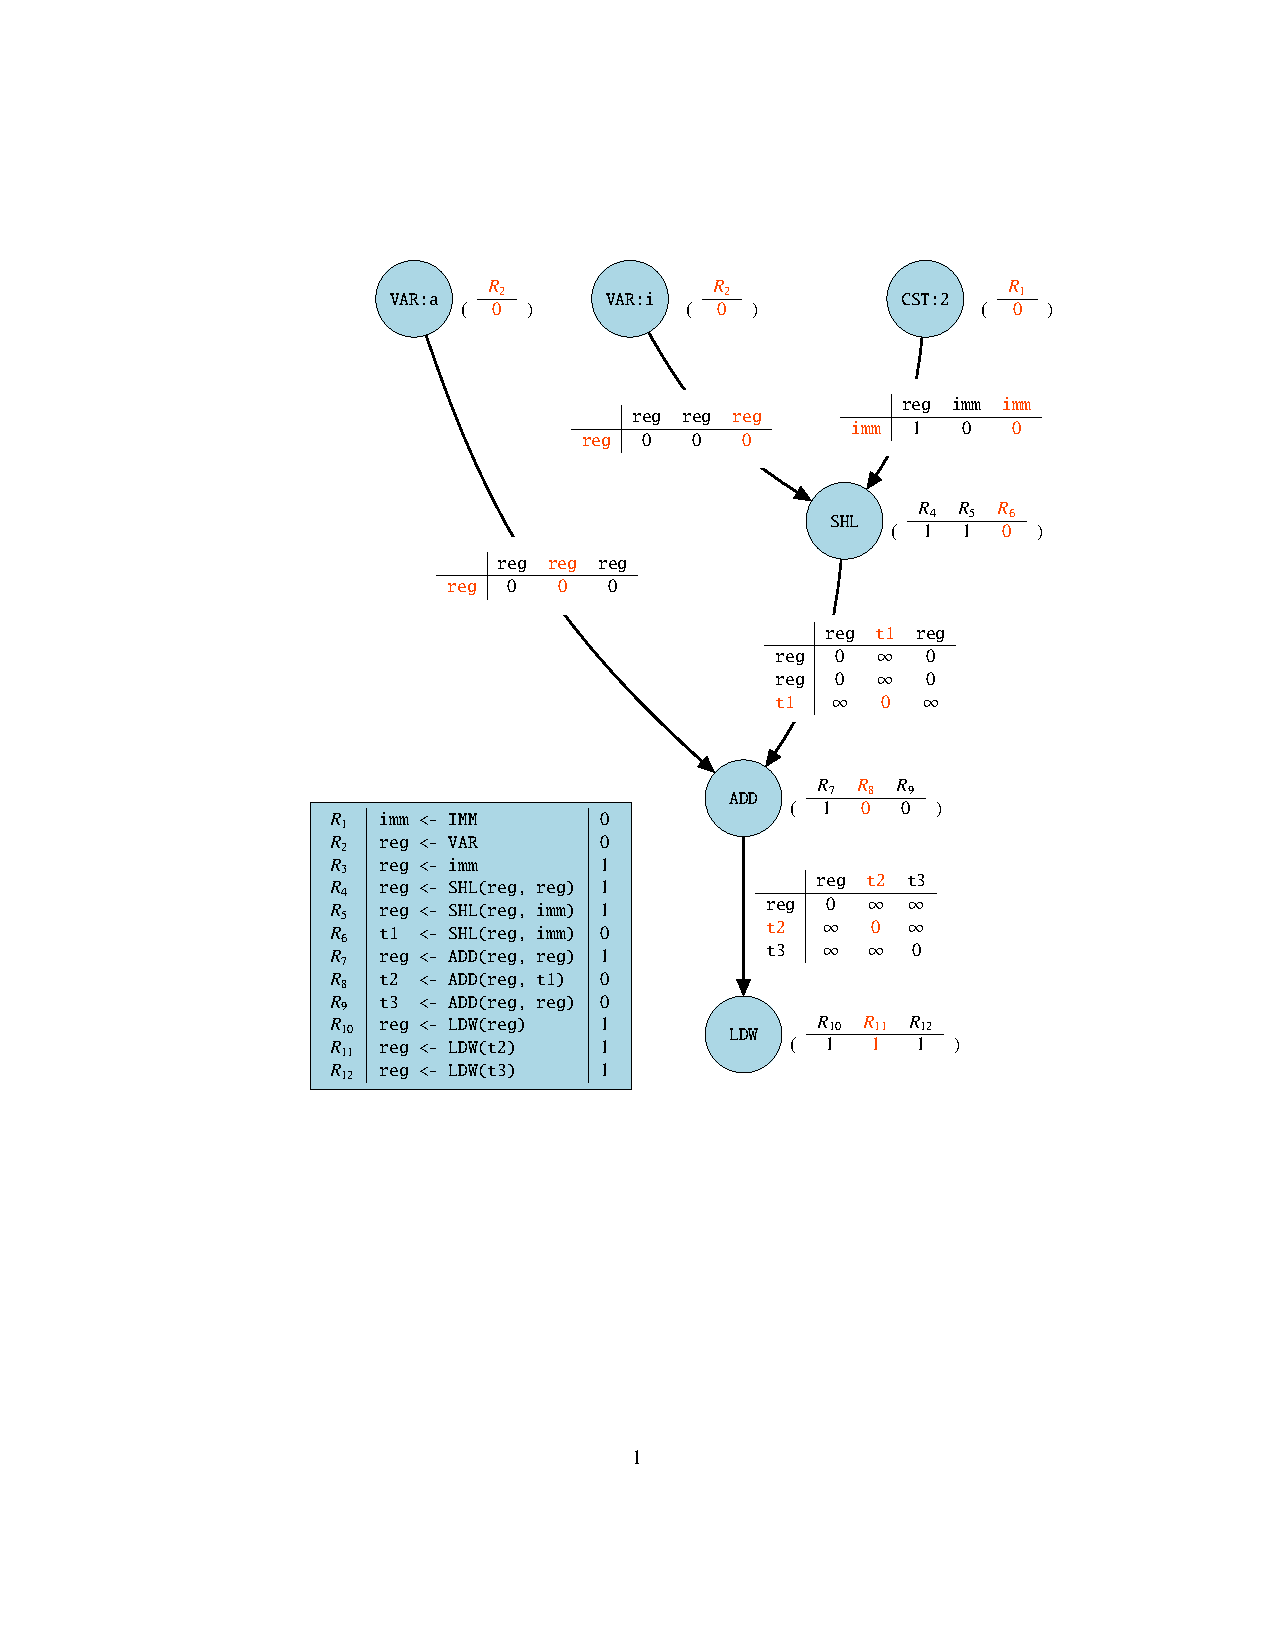
\includegraphics{pgf-fig006}
  \end{center}
  \caption{PBQP instance derived from the example shown in
    Figure~\ref{fig:tpm}. The grammar has been normalized by
    introducing additional nonterminals.}\label{fig:pbpq-example}
\end{figure}


The instruction selection problem for SSA graphs is modeled in PBQP as
follows. For each node $u$ in the SSA graph, a PBQP variable $x_u$ is
introduced. The domain of variable $x_u$ is determined by the subset
of base rules whose terminal symbol matches the operation of the SSA
node, \eg there are three rules ($R_4$, $R_5$, $R_6$) that can be
used to cover the shift operation $\texttt{SHL}$ in our example. The
last rule is the result of automatic normalization of a more complex
tree pattern.
The cost vector $\vec{c_u}= w_u \cdot \langle c(R_1), \dots,
c(R_{k_u}) \rangle$ of variable $x_u$ encodes the local costs for a
particular assignment where $c(R_i)$ denotes the associated cost of
base rule $R_i$. Weight $w_u$ is used as a parameter to optimize for
various objectives including speed (e.g. $w_u$ is the expected
execution frequency of the operation at node $u$) and space (e.g. the
$w_u$ is set to one). In our example, both $R_4$ and $R_5$ have
associated costs of one. Rule $R_6$ contributes no local costs as we
account for the full costs of a complex tree pattern at the root
node. All nodes have the same weight of one, thus the cost vector for
the \texttt{SHL} node is $\langle1, 1, 0 \rangle$.

An edge in the SSA graph represents data transfer between the result
of an operation $u$, which is the source of the edge, and the operand
$v$ which is the tail of the edge.  To ensure consistency among base
rules and to account for the costs of chain rules, we impose costs
dependent on the selection of variable $x_u$ and variable $x_v$ in the
form of a cost matrix $\matrixfont C_{uv}$. An element in the matrix
corresponds to the costs of selecting a specific base rule $r_u \in
R_u$ of the result and a specific base rule $r_v \in R_v$ of the
operand node. Assume that $r_u $ is $\texttt{nt} \leftarrow
\textit{op} (\dots)$ and $r_v$ is $\dots \leftarrow \textit{op}
(\alpha, \texttt{nt}', \beta)$ where $\texttt{nt'}$ is the
non-terminal of operand $v$ whose value is obtained from the result of
node $u$. There are three possible cases:
\begin{enumerate}
\item If the nonterminal \texttt{nt} and \texttt{nt}' are identical,
  the corresponding element in matrix $\matrixfont C_{uv}$ is zero,
  since the result of $u$ is compatible with the operand of node $v$.
\item If the nonterminals \texttt{nt} and $\texttt{nt}'$ differ and
  there exists a rule $r: \texttt{nt}' \leftarrow \texttt{nt}$ in the
  transitive closure of all chain-rules, the corresponding element in
  $\matrixfont C_{uv}$ has the costs of the chain rule, \ie $w_v \cdot
  c(r)$.
\item Otherwise, the corresponding element in $\matrixfont C_{uv}$ has
  infinite costs prohibiting the selection of incompatible base rules.
\end{enumerate}

As an example, consider the edge from \texttt{CST:2} to node
\texttt{SHL} in Figure~\ref{fig:pbpq-example}. There is a single base
rule $R_1$ with local costs 0 and result nonterminal \texttt{imm} for
the constant. Base rules $R_4$, $R_5$, and $R_6$ are applicable for
the shift, of which the first one expects nonterminal \texttt{reg} as
its second argument, rules $R_5$ and $R_6$ both expect
\texttt{imm}. Consequently, the corresponding cost matrix accounts for
the costs of converting from \texttt{reg} to \texttt{imm} at index
$(1,1)$ and is zero otherwise.

Highlighted elements in Figure~\ref{fig:pbpq-example} show a
cost-minimal solution of the PBQP with costs one. A solution of the
PBQP directly induces a selection of base and chain rules for the SSA
graph. A traversal over the basic blocks using the SSA graph is
sufficient to execute the associated semantic rules in order to emit
the code.

\section{Extensions and Generalizations}

\subsection{Code Selection for DAG Patterns}
% TODO (continue here)
\label{sec:dag_patterns}
% generalization for DAG patterns; motivation; modeling; example
In the previous section we have introduced an approach whose
patterns resemble simple tree fragments, \eg there is not support for
machine instructions with multiple results. This restricts the
modeling of advanced features commonly found in embedded
architectures and SIMD extensions of nowadays CPUs.

Consider the introductory example shown
in Figure~\ref{fig:ssa_graph}. Most architectures have some form of
auto-increment addressing modes. On such a machine, the load and the
increment of both \texttt{p} and \texttt{q} can be done in a single
instruction benefiting both code size and performance. However,
post-increment loads cannot be modeled using a single tree-shaped
pattern. Instead, it produces multiple results and spans across two
non-adjacent nodes in the SSA graph, with the only restriction that
their arguments have to be the same.

Similar examples can be found in most architectures, \eg the
\texttt{DIVU} instruction in the Motorola 68K architecture performs
the division and the modulo operation for the same pair of
inputs. Other examples are the \texttt{RMS} (read-modify-store)
instructions on the IA32/AMD64 architecture, autoincrement- and
decrement addressing modes of several embedded systems architectures,
the \texttt{IRC} instruction of the HPPA architecture, or
\texttt{fsincos} instructions of various math libraries. Compiler
writers are forced to pre- or post-process these patterns
heuristically often missing much of the optimization potential
\cite{Ebner08}. These architecture-specific tweaks also complicate
re-targeting, especially in situations where patterns are
automatically derived from generic architecture descriptions.

Supporting these patterns, however, is complicated by dependency
constraints among complex patterns. For any graph cover, the existence
of a topological order is necessary in order to generate correct
code. Cycles would imply that operations are executed on the target
hardware before the values of the operands are available. The partial
order among nodes is defined by the edges in the SSA graph and
eventual memory dependencies.

\begin{figure}
  \begin{center}
    \begin{tabular}{cc}
      \begin{minipage}[c]{4cm}
        \begin{tabbing}
          xx\=xxx\=xxx\=xxx\=\kill
          \texttt{(1) x$_\texttt{1}$:=*p;} \\
          \texttt{(2) *q:=1;} \\
          \texttt{(3) x$_\texttt{2}$:=x$_\texttt{1}$+1;} \\
          \texttt{(4) *p:=x$_\texttt{2}$;}
        \end{tabbing}
      \end{minipage}
      &
      \begin{minipage}[c]{\linewidth-4cm}
        \centering
%         \begin{tikzpicture}
%           \matrix [draw, rounded corners, fill=LightGrey, inner sep=10pt] (m) {
%             \node [fnode, inner sep=0] (st1) {\texttt{ST}};
%             \node [fnode, inner sep=0, below right of=st1, node distance=1.5cm] (inc) {\texttt{INC}};
%             \node [fnode, inner sep=5pt, below left of=inc, node distance=1.5cm] (ld) {\texttt{LD}};
%             \\
%           };

%           \node [fnode, below left of=ld,node distance=2.5cm] (p) {\texttt{VAR:p}} ;
%           \node [fnode, below right of=ld, node distance=2.5cm,xshift=1.5cm] (st2) {\texttt{ST}};
%           \node [fnode, below left of=st2] (q) {\texttt{VAR:q}};
%           \node [fnode, below right of=st2] (1) {\texttt{1}};

%           \path (m.north west) node [anchor=south west] {RMS Pattern};
%           \path [arrow,->] (ld) -- (inc);
%           \path [arrow,->] (inc) -- (st1);
%           \path [arrow,->] (1) -- (st2);
%           \path [arrow,->] (q) -- (st2);
%           \path [arrow,->] (p) -- (ld);
%           \path [arrow,->] (p) edge [bend left=20] (st1);

%           \node [below right of=ld,node distance=1.5cm] (c1) {};
%           \node [left of=st2,node distance=1cm,yshift=0.5cm] (c2) {};
%           \path [arrow,dashed,->] (ld) .. controls (c1.center) and
%           (c2.center) .. node [fill=white] {\texttt{WAR}}  (st2);

%           \node [above  of=st2,node distance=2cm,xshift=10pt] (c1) {};
%           \node [right of=st1,node distance=3.5cm] (c2) {};
%           \path [arrow,dashed,->] (st2) .. controls (c1.center) and
%           (c2.center) .. node [fill=white] {\texttt{WAW}}  (st1);
%         \end{tikzpicture}
        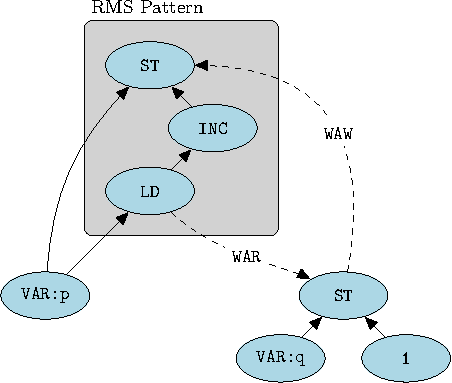
\includegraphics{pgf-fig007}
      \end{minipage}
      \\
      \\
      (a) Input Block &  (b) SSA Graph \\
    \end{tabular}
  \end{center}
  \caption{Potential memory dependencies for a tree-shaped
    read-modify-store (RMS) pattern.}\label{fig:rms}
\end{figure}

In principle, such issues can even arise for tree-shaped patterns. An
example is given in Figure~\ref{fig:rms}, which shows a typical
read-modify-store (RMS) pattern (``\texttt{add~r/m32,~imm32}'') for
the IA32/AMD64 architecture. A corresponding production rule might be
formulated as
\begin{alltt}
  stmt <- ST(\textit{x}:reg, ADD(LD(\textit{x}), imm)).
\end{alltt}
If we have to assume that \texttt{p} and \texttt{q} might address the
same memory location, we have to account for the antidependency among
statements \texttt{(1)} and \texttt{(2)} and the output dependency
among statements \texttt{(2)} and \texttt{(4)}; depicted in
Figure~\ref{fig:rms}\emph{(b)\/} by dotted lines. There is obviously
no topological order among the highlighted part forming the RMS
pattern and the store corresponding to instruction~\texttt{(2)}. Thus,
we cannot apply the pattern without introducing cyclic dependencies.

\begin{figure}[t]
  \centering
%   \begin{tikzpicture}

%     \node [anchor=south west] at (-5cm, 1cm) (listing) {
%       \begin{minipage}[]{7cm}
%         \begin{tabbing}
%           xx\=xxx\=xxx\=xxx\=\kill
%           \texttt{*p:=r+1;} \\
%           \texttt{*q:=p+1;} \\
%           \texttt{*r:=q+1;} \\
%         \end{tabbing}
%       \end{minipage}
%     };

%     \tikzstyle{mstyle}= [matrix,draw, fill=LightGrey, rounded
%     corners,column sep=10pt,row sep=10pt,inner sep=8pt];
%     \node[regular polygon, regular polygon sides=3, minimum size=4.5cm] (frame) {};

%     \path (frame.corner 2) node [mstyle] (m1) {
%       \node [fnode, inner sep=0] (st1) {\texttt{ST}}; \\
%       \node [fnode, inner sep=0] (inc1) {\texttt{INC}}; \\
%     };

%     \path (frame.corner 3) node [mstyle] (m2) {
%       \node [fnode, inner sep=0] (inc2) {\texttt{INC}}; \\
%       \node [fnode, inner sep=0] (st2) {\texttt{ST}}; \\
%     };

%     \path (frame.corner 1) node [mstyle, yshift=-0.8cm] (m3) {
%       \node [fnode, inner sep=0] (inc3) {\texttt{INC}}; &
%       \node [fnode, inner sep=0] (st3) {\texttt{ST}}; \\
%     };

%     \node [fnode, left of=m1,node distance=2.5cm] (q) {\texttt{VAR:q}};
%     \node [fnode, right of=m2,node distance=2.5cm] (r) {\texttt{VAR:r}};
%     \node [fnode, above of= m3,node distance=1.5cm] (p) {\texttt{VAR:p}};

%     \path [arrow,->] (inc1) -- (st2);
%     \path [arrow,->] (inc2) edge[bend right=15pt] (st3);
%     \path [arrow,->] (inc3) edge[bend right=15pt] (st1);

%     \path [arrow,->] (q) edge[bend right=5pt] (inc1);
%     \path [arrow,->] (q) edge[bend left=5pt] (st1);
%     \path [arrow,->] (r) edge[bend left=5pt] (st2);
%     \path [arrow,->] (r) edge[bend right=5pt] (inc2);
%     \path [arrow,->] (p) edge[bend right=5pt] (inc3);
%     \path [arrow,->] (p) edge[bend left=5pt] (st3);

%   \end{tikzpicture}
    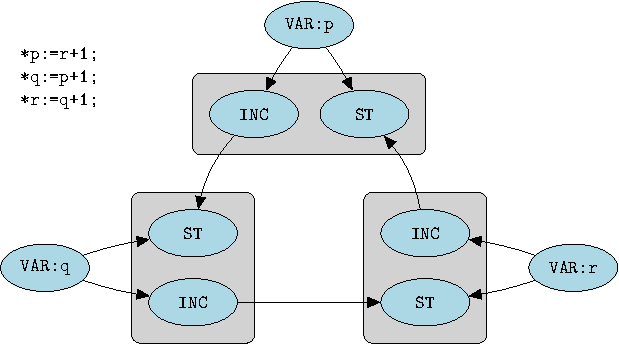
\includegraphics{pgf-fig008}
  \caption{DAG patterns may introduce cyclic data dependencies.}\label{fig:topology}
\end{figure}

However, for tree-shaped patterns, we can always perform a
\emph{local} check that determines if a particular pattern is or is
not applicable. For DAG patterns, this is not necessarily the
case. Again, an example is given in Figure~\ref{fig:topology}.  The
code fragment contains three feasible examples of a post-increment
store pattern. Assuming that we know that $p$, $q$, and $r$ point to
mutually distinct memory locations, there are no further dependencies
apart from the edges shown in the SSA graph.  However, the situation
is now different.  The example gives rise to a topological order as
long as we do not select \emph{all} three instances of the
post-increment store pattern concurrently. Thus, the existence of a
topological order is now a global property, which has to be considered
in the modeling of the problem.

\begin{algorithm}
\caption{Generalized PBQP instruction selection}
\label{alg:pbqpisel}
\begin{algorithmic}[1]
  \STATE identify instances of complex patterns within basic blocks
  \STATE transform the problem to an instance of PBQP
  \STATE obtain a solution for the PBQP instance using a generic
  solver
  \FORALL{basic blocks $b$}
    \STATE compute a topological order for the subgraph
    induced by basic block $b$
    \STATE apply the semantic rules associated with the chosen
    productions in the order computed in step \texttt{(5)}.
  \ENDFOR
\end{algorithmic}
\end{algorithm}

A proper generalization of the PBQP based instruction selection
\cite{Ebner08} is outlined in Algorithm~\ref{alg:pbqpisel}. Only steps
\texttt{(1)}, \texttt{(2)}, and \texttt{(5)} differ from the approach
discussed so far. First, we identify concrete tuples of nodes in the
SSA graph that can be used to form complex patterns. Next, we
transform the problem to an instance of PBQP that is processed using a
generic solver library. The problem formulation ensures the existence
of a topological order among the chosen productions and allows for a
straight-forward back-transformation that maps a solution vector of
PBQP to a complete graph cover. The partial order among the particular
nodes is defined by the edges in the SSA graph and additional data
dependencies among load and store instructions.  We can thus use a
reversed post-order traversal to apply the semantic actions associated
with the chosen productions in a proper order on the subgraphs induced
by individual basic blocks.

\subsubsection{Modeling}
As for tree patterns, DAG patterns are decomposed into simple base
rules for the purpose of modeling, \eg the postincrement store
pattern
\begin{alltt}
  P1: tmt <- ST(\textit{x}:reg, reg), reg <- INC(\textit{x}) : 3
\end{alltt}
is decomposed into the individual pattern fragments
\begin{alltt}
  P1.1: stmt <- ST(reg, reg)
  P1.2: reg  <- INC(reg)
\end{alltt}
The matcher explicitly enumerates \emph{instances\/} of complex
patterns in step \texttt{(1)} of Algorithm~\ref{alg:pbqpisel}, \ie
concrete tuples of nodes that match the terminal symbols specified in
a particular production. In the example shown in
Figure~\ref{fig:topology}, there are three instances of the
postincrement store pattern. Dependencies among these instances
(denoted in the following by $\prec$) arise from real dependencies
among individual nodes (edges in the SSA graph) and eventual memory
dependencies as outlined in Figure~\ref{fig:rms}.
For instances of DAG patterns, additional decision variables are
required that encode if the particular pattern is to be
selected. Thus, we have two sets of decision variables
$X=X_1~\dotcup~X_2$ for regular SSA nodes and instances of complex
patterns respectively.

The domain for variables in $X_1$ is defined by the set of applicable
base rules arising from two different sources:
\begin{enumerate}
\item Simple productions consisting of a single base rule; these are
  handled just like before for tree grammars.
\item Base rules arising from the decomposition of DAG patterns. All
  identical base rules obtained from the decomposition of complex
  productions contribute only to a single element in the decision
  vector.
\end{enumerate}
While the former group represents the set of simple patterns that can
be used to obtain a cover for a particular node, the second class of
base rules can be seen as a proxy for the whole set of instances of
(possibly different) complex productions including the node. The
costs for these proxy states are $0$, otherwise they reflect the
real costs of the corresponding tree rule.

Variables in set $X_2$ are created for each enumerated instance of a
complex production. They encode whether a particular instance is
chosen or not, \ie the domain basically consists of the elements
\textit{on} and \textit{off}. The local costs reflect the costs for
the particular pattern except for the \textit{off} state, which is set
to $0$.

\begin{figure}
  \centering
%   \begin{tikzpicture}[]

%     \tikzstyle{mstyle}= [matrix,draw, fill=LightGrey, rounded corners,
%     column sep=10pt,row sep=10pt,inner sep=8pt];
%     \tikzstyle{nstyle}= [draw,fill=LightBlue,shape=rectangle,rounded corners,inner sep=2pt];

%     \node[regular polygon, regular polygon sides=3, minimum size=3.3cm] (frame) {};

%     \path (frame.corner 1) +(0,0) node  (ci1) [nstyle, yshift=0.6cm]
%     {
%       \begin{tabular}{@{}c@{}}
%         7: instance $\langle 2,1 \rangle$ \\
%         \hline
%         $\begin{array}{cccccc}
%           & \texttt{off} & \texttt{on}_1 & \texttt{on}_2 & \texttt{on}_3 & \\
%           ( & 0 & k & k & k & )
%         \end{array}$
%       \end{tabular}
%     };

%     \path (frame.corner 2) +(-1.5,0) node  (ci2) [nstyle]
%     {
%       \begin{tabular}{@{}c@{}}
%         8: instance $\langle 3,4 \rangle$ \\
%         \hline
%         $\begin{array}{cccccc}
%           & \texttt{off} & \texttt{on}_1 & \texttt{on}_2 & \texttt{on}_3 & \\
%           ( & 0 & k & k & k & )
%         \end{array}$
%       \end{tabular}
%     };

%     \path (frame.corner 3) +(1.5,0) node  (ci3) [nstyle]
%     {
%       \begin{tabular}{@{}c@{}}
%         9: instance $\langle 5,6 \rangle$ \\
%         \hline
%         $\begin{array}{cccccc}
%           & \texttt{off} & \texttt{on}_1 & \texttt{on}_2 & \texttt{on}_3 & \\
%           ( & 0 & k & k & k & )
%         \end{array}$
%       \end{tabular}
%     };

%     \path (frame.corner 2) +(-1,-4.5) node [mstyle] (m1)
%     {
%       \node  (st1) [nstyle]
%       {
%         \begin{tabular}{@{}c@{}}
%           3: \texttt{ST} \\
%           \hline
%           $(\, \texttt{P2} \quad \texttt{P1.1}\, )$\\
%           $(\, 2 \quad \texttt{M} \,)$ \\
%         \end{tabular}
%       };
%       &

%       \node  (inc1) [nstyle]
%       {
%         \begin{tabular}{@{}c@{}}
%           4: \texttt{INC} \\
%           \hline
%           $(\, \texttt{P3} \quad \texttt{P1.2}\, )$\\
%           $(\, 2 \quad \texttt{M} \,)$ \\
%         \end{tabular}
%       };

%       \\
%     };

%     \path (frame.corner 3) +(1,-4.5) node [mstyle] (m2)
%     {
%       \node  (st2) [nstyle]
%       {
%         \begin{tabular}{@{}c@{}}
%           5: \texttt{ST} \\
%           \hline
%           $(\, \texttt{P2} \quad \texttt{P1.1}\, )$\\
%           $(\, 2 \quad \texttt{M} \,)$ \\
%         \end{tabular}
%       };
%       &

%       \node  (inc2) [nstyle]
%       {
%         \begin{tabular}{@{}c@{}}
%           6: \texttt{INC} \\
%           \hline
%           $(\, \texttt{P3} \quad \texttt{P1.2}\, )$\\
%           $(\, 2 \quad \texttt{M} \,)$ \\
%         \end{tabular}
%       }; \\
%     };

%     \path (frame.corner 1) +(0,4.5) node [mstyle] (m3)
%     {
%       \node  (inc3) [nstyle]
%       {
%         \begin{tabular}{@{}c@{}}
%           1: \texttt{INC} \\
%           \hline
%           $(\, \texttt{P3} \quad \texttt{P1.2}\, )$\\
%           $(\, 2 \quad \texttt{M} \,)$ \\
%         \end{tabular}
%       };
%       &
%       \node  (st3) [nstyle]
%       {
%         \begin{tabular}{@{}c@{}}
%           2: \texttt{ST} \\
%           \hline
%           $(\, \texttt{P2} \quad \texttt{P1.1}\, )$\\
%           $(\, 2 \quad \texttt{M} \,)$ \\
%         \end{tabular}
%       };
%       \\
%     };

%     \node [fnode, below of=m1,node distance=1.8cm] (q) {\texttt{VAR:q}};
%     \node [fnode, below of=m2,node distance=1.8cm] (r) {\texttt{VAR:r}};
%     \node [fnode, above of=m3,node distance=1.8cm] (p) {\texttt{VAR:p}};

%     \path [arrow,->] (q) -- (inc1);
%     \path [arrow,->] (q) -- (st1);
%     \path [arrow,->] (r) -- (st2);
%     \path [arrow,->] (r) -- (inc2);
%     \path [arrow,->] (p) -- (inc3);
%     \path [arrow,->] (p) -- (st3);

%     \path[arrow,->] (inc1) edge[bend right=60pt] node[yshift=-0.6cm] {$\left( { \begin{array}{cc}
%             0 & 0 \\
%             0 & 0 \\
%           \end{array}} \right)$} (st2);

%     \path [arrow,->] (inc2.east) .. controls
%     ($(inc2)+(3.2cm,2cm)$) and ($(st3)+(4cm,-2cm)$) ..
%     node[fill=white,near end] {$\left( { \begin{array}{cc}
%             0 & 0 \\
%             0 & 0 \\
%           \end{array}} \right)$} (st3.east);

%     \path [arrow,->] (inc3.west) .. controls ($(inc3)+(-4cm,-2cm)$) and
%     ($(st1)+(-3.2cm,2cm)$) ..
%     node[fill=white,near start] {$\left( { \begin{array}{cc}
%             0 & 0 \\
%             0 & 0 \\
%           \end{array}} \right)$} (st1.west);

%     \path[arrow,->] (ci2) edge[bend right=10] node[fill=white] {$\left( { \begin{array}{cccc}
%             0 & 0 & 0 & 0 \\
%             0 & \infty & 0 & 0 \\
%             0 & \infty & \infty & 0 \\
%             0 & \infty & \infty & \infty \\
%           \end{array}} \right)$} (ci3);

%     \path[arrow,->] (ci3) edge[bend right=60] node[fill=white] {$\left( { \begin{array}{cccc}
%             0 & 0 & 0 & 0 \\
%             0 & \infty & 0 & 0 \\
%             0 & \infty & \infty & 0 \\
%             0 & \infty & \infty & \infty \\
%           \end{array}} \right)$} (ci1.east);

%     \path[arrow,<-] (ci2) edge[bend left=60] node[fill=white] {$\left( { \begin{array}{cccc}
%             0 & 0 & 0 & 0 \\
%             0 & \infty & 0 & 0 \\
%             0 & \infty & \infty & 0 \\
%             0 & \infty & \infty & \infty \\
%           \end{array}} \right)$} (ci1.west);

%     \path[arrow,->] (inc3) edge[bend right=30] node[fill=white] {$\left( { \begin{array}{cccc}
%             0 & \infty & \infty & \infty \\
%             0 & 0 & 0 & 0 \\
%           \end{array}} \right)$} (ci1);


%     \path[arrow,->] (st3) edge[bend left=30] node[fill=white] {$\left( { \begin{array}{cccc}
%             0 & \infty & \infty & \infty \\
%             0 & 0 & 0 & 0 \\
%           \end{array}} \right)$} (ci1);


%     \path[arrow,->] (inc1) edge[bend right=30] node[fill=white] {$\left( { \begin{array}{cccc}
%             0 & \infty & \infty & \infty \\
%             0 & 0 & 0 & 0 \\
%           \end{array}} \right)$} (ci2);


%     \path[arrow,->] (st1) edge[bend left=30] node[fill=white] {$\left( { \begin{array}{cccc}
%             0 & \infty & \infty & \infty \\
%             0 & 0 & 0 & 0 \\
%           \end{array}} \right)$} (ci2);

%     \path[arrow,->] (inc2) edge[bend right=30] node[fill=white] {$\left( { \begin{array}{cccc}
%             0 & \infty & \infty & \infty \\
%             0 & 0 & 0 & 0 \\
%           \end{array}} \right)$} (ci3);


%     \path[arrow,->] (st2) edge[bend left=30] node[fill=white] {$\left( { \begin{array}{cccc}
%             0 & \infty & \infty & \infty \\
%             0 & 0 & 0 & 0 \\
%           \end{array}} \right)$} (ci3);


%   \end{tikzpicture}
    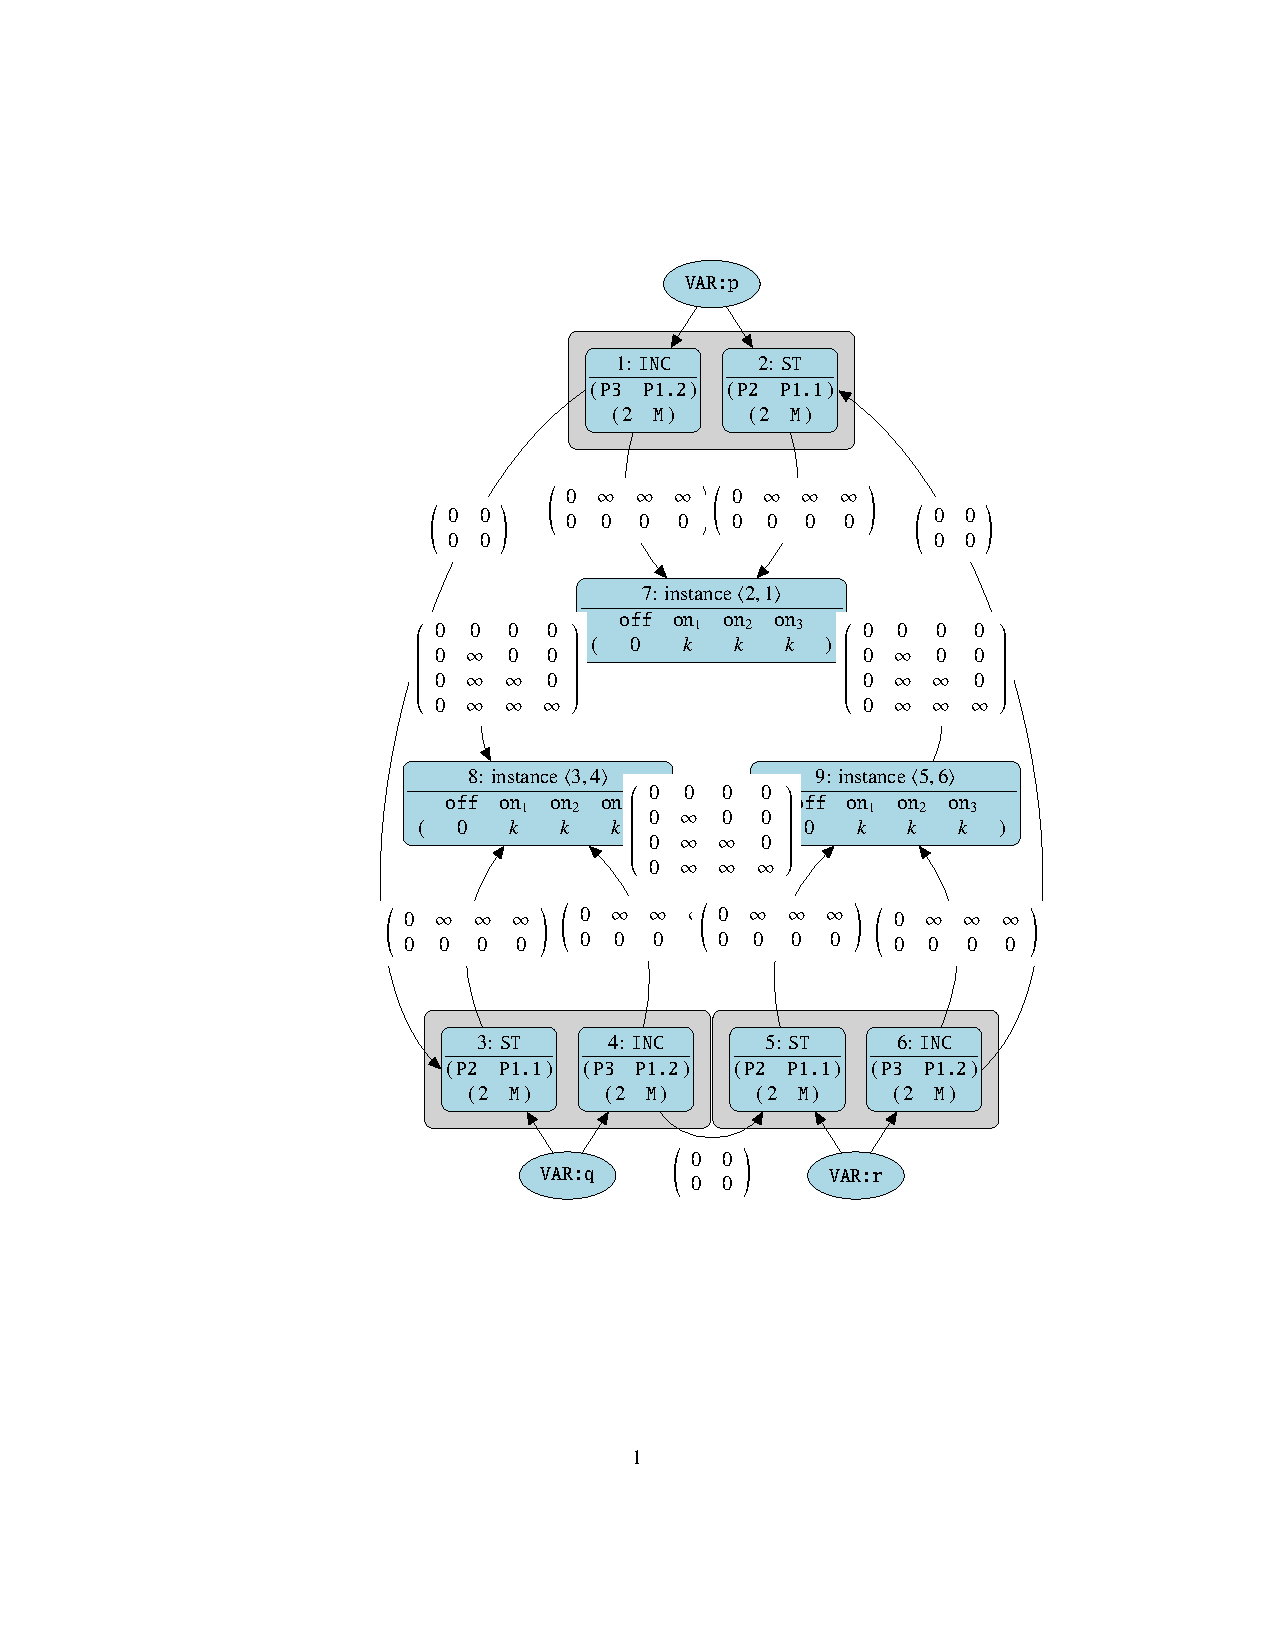
\includegraphics{pgf-fig009}
  \caption{PBQP Graph for the Example shown in
    Figure~\ref{fig:topology}. We use $k$ as a shorthand for the term
    $3-2M$.}\label{fig:pbqpinst}
\end{figure}

The PBQP for the SSA graph introduced in Figure~\ref{fig:topology} is
shown in Figure~\ref{fig:pbqpinst}. In addition to the postincrement
store pattern with costs 3, we assume regular tree patterns for the
store and the increment nodes with costs two denoted by \texttt{P2}
and \texttt{P3} respectively. Rules for the \texttt{VAR} nodes are
omitted for simplicity.

Nodes one to six correspond to the nodes in the SSA graph. Their
domain is defined by the simple base rule with costs two and the proxy
state obtained from the decomposition of the postincrement store
pattern. Nodes 7, 8, and 9 correspond to the three instances
identified for the postincrement store pattern. As noted before, we
have to guarantee the existence of a topological order among the
chosen nodes.  One approach is to exploit the property that every
acyclic directed subgraph gives rise to a not necessarily unique
topological order.  We can refine the state \textit{on} such that it
reflects a particular index in a concrete topological order. Matrices
among these nodes account for data dependencies, \eg consider the
matrix established among nodes 7 and 8. Assuming instance 7 is
\textit{on} at index 2, the only remaining choices for instance 8 are
not to use the pattern or to enable it at index three, as node 7 has
to precede node 8.

A different class of constraint matrices is required to ensure that
the corresponding proxy state is selected on all the variables forming
a particular pattern instance. Therefore, we create matrix costs
$C^{X_1 \rightarrow X_2}_{ul}$ such that the costs are zero if $x_l$
is set to \textit{off\/} or $x_u$ is set to a base rule that is not
associated to the instance. Otherwise, costs are set to $\infty$.
Thus, when one of the instances correlated to a particular node $u$ in
the SSA graph is selected, the only remaining element in the domain of
$u$ with costs less than $\infty$ is the associated proxy state
corresponding to the particular base rule fragment.

So far, the formulation allows the trivial solution where all of the
related variables encoding the selection of a complex pattern are set
to \textit{off} (accounting for 0 costs) even though the artificial
proxy state has been selected. We can overcome this problem by adding
a large integer value $M$ to the costs for all proxy states. In
exchange, we subtract these costs from the cost vector of
instances. Thus, the penalties for the proxy states are effectively
eliminated unless an invalid solution is selected.
Cost matrices among nodes one to six do not differ from the basic
approach discussed before and reflect the costs of converting the
nonterminal symbols involved.
It should be noted that for general grammars and irreducible graphs,
that the heuristic solver of PBQP cannot guarantee to deliver a solution 
that satisfies all constraints modeled in terms of $\infty$ costs. This would be a
NP-complete problem. One way to work around this limitation is to
include a small set of rules that cover each node individually and
that can be used as a fallback rule in situations where no feasible
solution has been obtained. This corresponds to macro substitution
techniques and ensures a correct but possibly suboptimal matching. In
practice, this is no severe limitation as grammars are usually written
by defining a simple but complete set of rules covering each node
individually and adding more complex rules later on. These limitations
do not apply to exact techniques such as the branch-\&-bound algorithm. 
It is also straight-forward
to extend the heuristic algorithm with a backtracking scheme on RN
reductions, which would clearly also be exponential in the worst case.

\subsection{Chain Rule Placement}
\label{sec:chain_rule_placement}
% \emph{1 page}; optimal chain rule placement
Chain rules can either be emitted at the basic block corresponding to
the source node or right before each use, \ie at the destination
node. In~\cite{1269857}, a more sophisticated technique is introduced
that allows a more efficient placement of chain rules across basic
block boundaries. This technique is orthogonal to the generalization
to complex patterns. An optimal placement is computed by the
construction of a min-cut problem for the given control flow graph. A
solution for this problem can be found in polynomial time. There is a
trade-off among performance and code size that is captured accurately
in the proposed network flow model.


\section{Summary}

Instruction selection on SSA-graph enables aggressive code
selection optimisations. The whole flow of a function is taken
into account rather a local scope. Hence, code selection
for SSA graphs goes beyond the state-of-the-art tree-pattern
matching techniques. 
For the compiler implementor the move from tree-pattern
matches to SSA matching is a small step as long as a
PBQP library and some basic infrastructure (graph grammar
translator, etc.) is provided. The complexity of the
approach is hidden in the discrete optimisation problem called
PBQP. Free PBQP libraries are available 
from the web-pages of the authors and a library is implemented
as part of the LLVM framework for register allocation. 

%%% Local Variables:
%%% mode: latex
%%% TeX-master: "chapter"
%%% End:
